%LTeX: language=de-DE
\chapter{Frontend}
Das Frontend ist jener Teil, der im Browser sichtbar ist und dient als Schnittstelle zwischen dem Anwender und den Daten. Es kann mithilfe einer Programmierschnittstelle (API) auf diese Daten zugreifen, um diese verändern oder anzeigen zu können. Für die Implementierung wurde die Bibliothek ''React\footnote{https://reactjs.org}'' verwendet. Im ''frontend/src'' Verzeichnis liegen drei Unterverzeichnisse: ''images'': Beinhaltet alle Abbildungen, die im Frontend angezeigt werden, ''scripts'': Beinhaltet den TypeScript und HTML Code zum Aufbau des Frontends, ''styles'': Beinhaltet die CSS Files für das Styling der Oberflächen. 

\section{Main.tsx}
Der Einstiegspunkt der React-App liegt im Verzeichnis ''frontend/src/scripts''. Das dort liegende File ''main.tsx'' [siehe Abb. \ref{fig: frontendmain} auf S.~\pageref{fig: frontendmain}] rendert das ''<Root/>'' Element der App, in dem dann die verschiedenen Views über den Router hineingerendert werden. Dafür wird zuerst ein ''root'' Element erstellt, dass an den ''body'' angefügt wird. Die ''ReactDom.render(element,container)'' Methode rendert dann das Element in das vorher erzeugte ''div'' Tag. Das Element, dass der ''render'' Methode mitgegeben wird beinhaltet zusätzlich noch den ''<Auth0Provider/>'' für das Anmelden über verschiedene Plattformen wie zum Beispiel dem Microsoft Account und den ''<BrowserRouter>'' für das Routing innerhalb des Frontends. Das ''<Helmet>'' Tag wird wie der ''<head>'' tag einer HTML Datei verwendet um Metadaten, wie das App-Icon, angeben zu können.

\begin{figure}[h]
    \centering
    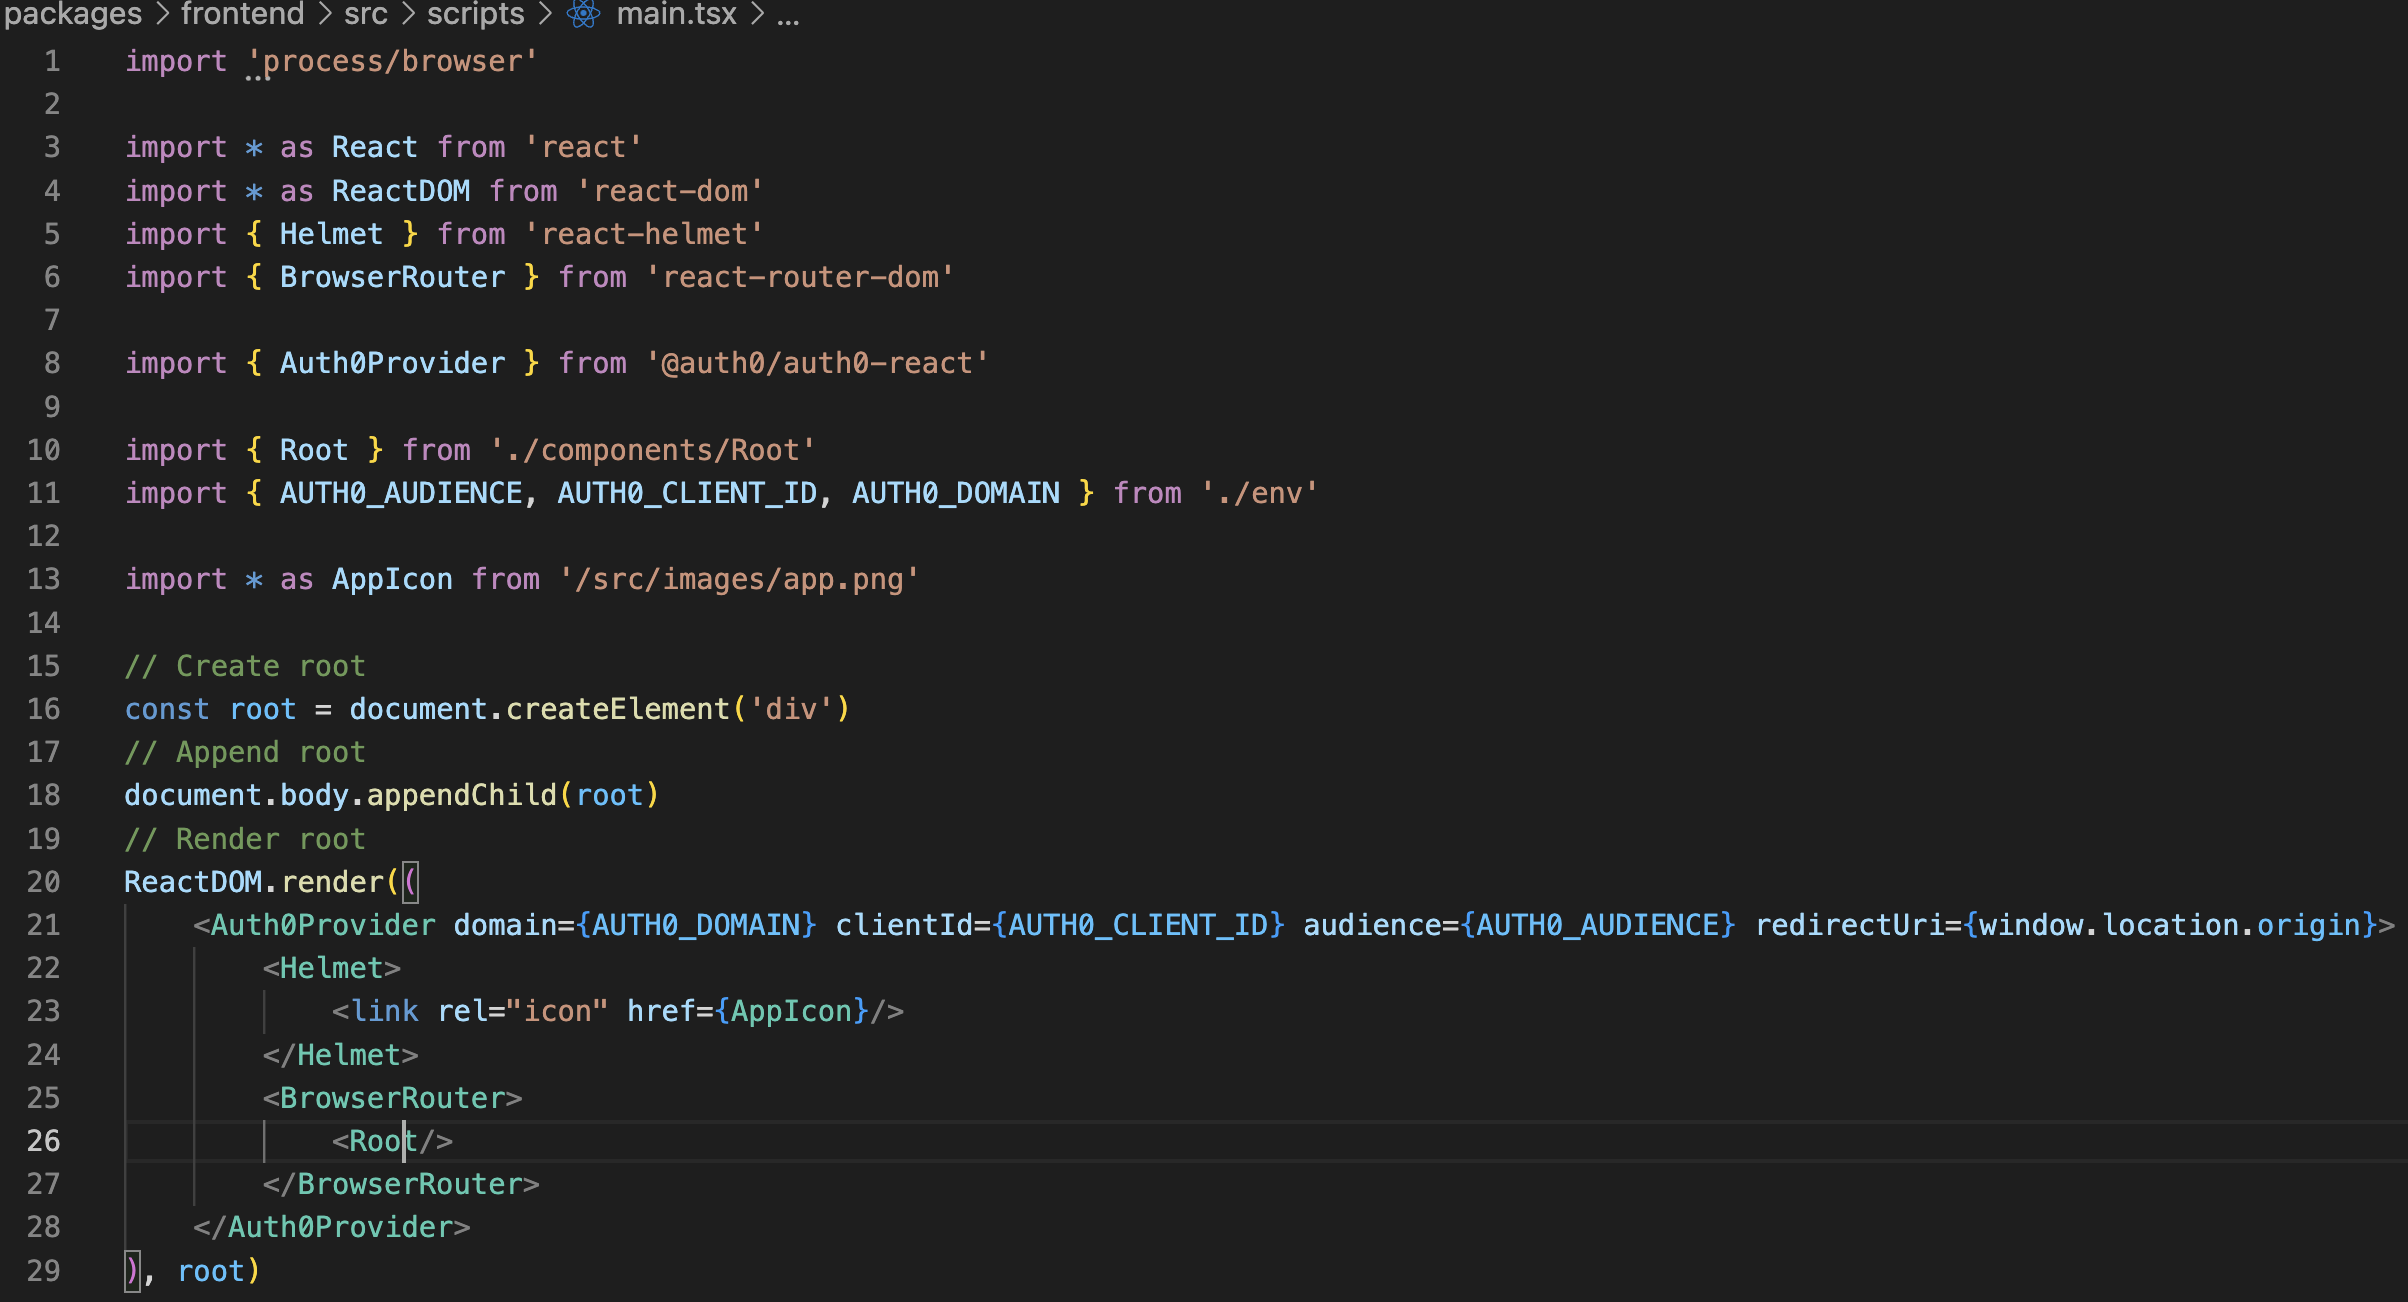
\includegraphics[width=1\textwidth]{frontendmain.png}
    \caption{main.tsx}
    \label{fig: frontendmain}
\end{figure}

\section{Root.tsx}
Im Verzeichnis ''frontend/src/scripts/components'' liegt die Datei ''Root.tsx''. Dabei handelt es sich um jene Komponente, die mit dem ''<Root/>'' tag in der ''main.tsx'' eingebunden wird. Die ''Root.tsx'' kümmert sich um das Authentifizieren des Users mit Auth0\footnote{https://auth0.com}, stellt für den User und die Produktversion eine globale Variable (useContext) bereit und definiert die Routen innerhalb der App. Bei den Routen wird definiert bei welcher URL im Browser, welche View gerendert werden soll.

\section{Aufbau der Views}
Im Verzeichnis ''frontend/src/scripts/components/views'' liegen alle Views, die mithilfe des React-Routers gerendert werden können. Dabei ist der Code jeder View ähnlich strukturiert: Ganz oben kommen die Imports und darunter wird die View in einer Arrowfunktion aufgebaut und exportiert. Dafür gibt es in jeder View folgende Bereiche:
\begin{itemize}
    \item REFERENCES: Hier wird der ''useRef'' Hook verwendet, um von einer funktionalen Komponente direkt auf ein DOM Element zugreifen zu können. So kann zum Beispiel auf einen Textinput zugegriffen werden um darauf den Fokus zu setzen.
    \item PARAMS: Sind Variablen, die aus der aktuellen URL entnommen werden, wie zum Beispiel die Produkt ID. 
	\item CONTEXTS: Globale States, die über das ganze Frontend hinweg ausgelesen und überschrieben werden können. So ist über alle Tabs hinweg der aktive User bekannt oder die eingestellte Version eines Produkts kann in allen Tabs angezeigt werden ohne diese neu einstellen zu müssen.
	\item INITIAL STATES: Hier werden Daten geholt, die bereits im Cache des Frontends vorhanden sind.
	\item STATES: Sind als ''useState'' realisiert und verhalten sich wie Properties, die gelesen und mit einer Methode beschrieben werden können. Ändert sich ein State, so wird der aktuelle Tab neu gerendert.
	\item EFFECTS: Hier werden die Daten mit ''useEffect(effect, deps)'' aus dem Backend geholt, wenn sich ein Wert in der jeweiligen DependencyList (deps) ändert. Eine leere DependencyList bedeutet, dass der ''useEffect'' beim Besuchen der Seite einmalig aufgerufen wird. 
	\item FUNCTIONS: In diesem Bereich sind Funktionen definiert, die anderswo im selben File aufgerufen werden können. Wie zum Beispiel das Löschen eines Produkts über einen Button.
	\item CONSTANTS: Definiert konstante Strukturen, wie zum Beispiel Tabellenspalten, die variabel mit den geladenen Daten befüllt werden können.
	\item RETURN: Hier ist der Rückgabewert der Arrowfunktion. In einem Return wird ein HTML Tag zurückgegeben, der verschiedene Kindelemente beinhalten kann. Der Inhalt der aktuellen Route wird dann von der ''ReactDOM.render'' Methode von der main.tsx auf dem Bildschirm dargestellt.
\end{itemize}
React bietet den Vorteil, dass sich eigene Komponenten erstellen lassen, die dann in anderen Komponenten wiederverwendet werden können. So wurden für die verschiedensten Anwendungsfälle bereits Komponenten erstellt, die in anderen Komponenten verwendet werden können. Es findet sich zum Beispiel im Verzeichnis ''frontend/src/scripts/components/widgets'' das File ''Table.tsx'', welches bei fast jeder View zum Einsatz kommt um die geladenen Daten tabellarisch anzeigen zu können. Diese Komponenten sind nach Kategorien unterteilt und liegen in ihren dafür erstellten Verzeichnissen. Die Kategorien sind dabei: inputs, links, snippets und widgets. 

\section{Zugriff auf die API}
Der Zugriff auf die API geschieht im Frontend über drei Ebenen. Hier sind, als Beispiel, die Stationen für das Auslesen der Produkte aufgezeigt:
\begin{enumerate}
	\item Aufruf in einer View über den jeweiligen Manager mit: ''ProductManager.findProducts(). then(setProducts)''. 
	\item Im jeweiligen Manager (''frontend/src/scripts/components/managers'') wird geprüft, ob die Produkte bereits im Cache liegen. Falls ja, werden sie vom Cache geholt und zurückgegeben. Falls nein, kommt es zur dritten Ebene.
	\item Die ''findProducts()'' Methode aus dem product.ts im Verzeichnis ''frontend/src/scripts/clients/rest'' aufrufen. Diese asynchrone Methode sendet mithilfe der Bibliothek ''Axios\footnote{https://axios-http.com}'' einen ''get'' Request an das Backend und gibt das Ergebnis als ''Promise'' zurück. Kommt dieses Promise an, so wird in der View mit ''...().then(setProducts) die Liste aus Produkten gesetzt.
\end{enumerate}

\section{Darstellung des 3D-CAD Modells}
Für die Darstellung des 3D-CAD Modells wird die Komponente ''<ProductView3D/>'' in den jeweiligen Views verwendet, die in sich die Komponente ''<VersionView3D/>'' trägt. ''<VersionView3D/>'' benutzt die Komponente ''<FileView3D/>'' um das gewünschte ''.glb\footnote{https://docs.fileformat.com/3d/glb/}'' File mithilfe der Bibliothek ''three.js\footnote{https://threejs.org}'' über die  ''<ModelView3D/>'' Komponente darzustellen. Diese Kaskade an Komponenten ermöglicht, dass auf oberster Ebene nur definiert werden muss welches Produkt oder welche Version dargestellt werden soll. Wird nur das Produkt angegeben, so sucht die ''<ProductView3D/>'' Komponente die aktuellste Version heraus und gibt sie weiter an die ''<VersionView3D/>''. Wird eine Version angegeben, so gibt die ''<ProductView3D/>'' die Version an die ''<VersionView3D/>'' weiter. Der''<FileView3D/>'' wird dann nur noch der Pfad der Datei übergeben. Diese verwendet dann die Komponente  ''<ModelView3D/>'', in der sich die Implementierung für die Anzeige der Modelle mittels ''three.js'' befindet.